\documentclass[a4paper, 12p]{article}
\usepackage[spanish]{babel} 
\usepackage{amsmath} 
\usepackage[colorlinks=true]{hyperref}
\usepackage{enumitem} 
\usepackage{graphicx}   
\usepackage[a4paper,top=3cm,bottom=3cm,left=3cm,right=3cm,marginparwidth=1.75cm]{geometry} 
\usepackage[]{subfigure}
\graphicspath{{./graficos/Lab-Termo/Git/Documentos}} 
\usepackage{float}
%\usepackage[]{txfonts}
\usepackage{multicol}



\newenvironment{Figura}
{\par\medskip\noindent\minipage{\linewidth}}
{\endminipage\par\medskip}

%==================================================================================
\begin{document}
\begin{titlepage}
      \begin{center}     
              
            
\includegraphics[width=0.2\textwidth]{img/escudo_udec.png}                       %Para poner logo udec   %{nombre carpeta\nombreimagen}
            
            
            
            \vspace{1cm}
            \textsc{{\LARGE Universidad de Concepción}}
            
            \vspace{1cm}
            {\scshape\Large Facultad de ciencias fisícas y matemáticas \par}
            \vspace{2cm}
            {\scshape\Huge Laboratorio 3 \par}
            \vspace{2cm}
            {\itshape\Large Proyecto laboratorio termodinámica \par}
            \vfill
            {\Large Autores: \par}
            {\Large Martina Contreras, Noemí De la peña, Benjamín Opazo. \par}
            \vfill
            \vfill
            {\Large Profesor: \par}
            {\Large Claudio Alonso Faúndez Araya \par}
            \vfill
            \vfill
            {\Large Carrera: \par}
            {\Large Ciencias fisícas \par}
            \vfill
            \vfill
            {\Large Ayudantes: \par}
            {\Large Arelly Nunez y Anahis Verana \par}
            \vfill
            {\Large Noviembre 2022 \par}
      \end{center}
\end{titlepage}            
%\maketitle  

\tableofcontents
\newpage

%========Introducción
\section{Introdución}


\section{Objetivos}
\begin{itemize}
      \item Determinar experimentalmente el calor específico de un trozo de metal (alumio, cobre ó acero).
      \item Comparar el valor determinado con los existentes en la literatura.
\end{itemize}



%=========Marco Teórico
\section{Marco Teórico} 

\begin{itemize}
      \item \textbf{Capacidad calorífica: }(a cualquier temperatura) se define como  el limite de C cuando $\varDelta T$ tiende a 0:
      \begin{align}
            C = \frac{d'Q}{dT}           \qquad \left[\frac{J}{K}\right]              
      \end{align}
      donde: \\ \\
      $d'Q = $ Representa un pequeño flujo de calor. \\
      $dT = $ Es el correspondiente al cambio de temperatura. 

      \item \textbf{Calor específico: } Capacidad calorífica por unidad de masa o mol.
      \begin{align}
            c = \frac{C}{n}   \quad \left[\frac{J}{Kilo\cdot molK}\right]  \qquad o  \qquad c = \frac{C}{m} \quad \left[\frac{J}{KgK}\right]
      \end{align}

      \item \textbf{Cantidad total de calor } que fluye en un sistema en cualquier proceso, viene dado por:
      \begin{align}
            Q = \int d'Q &= \int_{T_i}^{T_F} C\cdot dT \\ \nonumber
                         &= \int_{T_i}^{T_F} mc\cdot dT
      \end{align}
      cuando c es constante, obtenemos que:
      \begin{align}
            Q = mc \, \varDelta T
      \end{align}

      \item \textbf{Calor latente o de transformación: } Es la razón del calor absorbido a la masa m que experimenta el cambio de fase. 
      \begin{align}
            l = \frac{Q}{m}                \qquad \left[\frac{J}{Kg}\right]
      \end{align}
      donde: \\ \\
      $Q$ = Es el flujo de calor necesario para que exista un cambio de fase.\\
      $n$ = moles

      \item \textbf{Cambio de fase: } se refiere a que una sustancia que absorve o cede calor sin que haya un cambio en su temperatura.
      \item \textbf{Calor latente de fusión: }es el calor requerido por unidad de masa para cambiar de un estado sólido a líquido a una presión y temperatura fija.
      \item \textbf{Calor latente de evaporación: } es el calor requerido por unidad de masa para pasar de un estado líquido a gaseoso a una presión y temperatura fija.
\end{itemize} 
Cada concepto fue extraído de \cite{libro}. \\

Nuestras hipótesis son:
\begin{enumerate}
      \item A mayor cantidad de sustancia, mayor será el tiempo en el que alcance el punto de ebullición.
      \item  A mayor potencia, la sustancia alcanza más rápido su punto de ebullición.
      \item A mismas condiciones iniciales, diferentes sustancias pueden alcanzar su punto de ebullición en distintos intervalos de tiempo.
      
      
\end{enumerate}


%=========Materiales
\section{Materiales}


\begin{itemize}
      \item Generador de vapor PASCO TD-8556A,
      \item Vaso precipitado,
      \item calorímetro,
       \item soporte universal,
      \item termómetros de mercurio x2,
      \item agua,
      \item balanza digital,
      \item trozo de metal.
\end{itemize}



\begin{figure}[H]
    \begin{subfigure}
          \raggedleft
          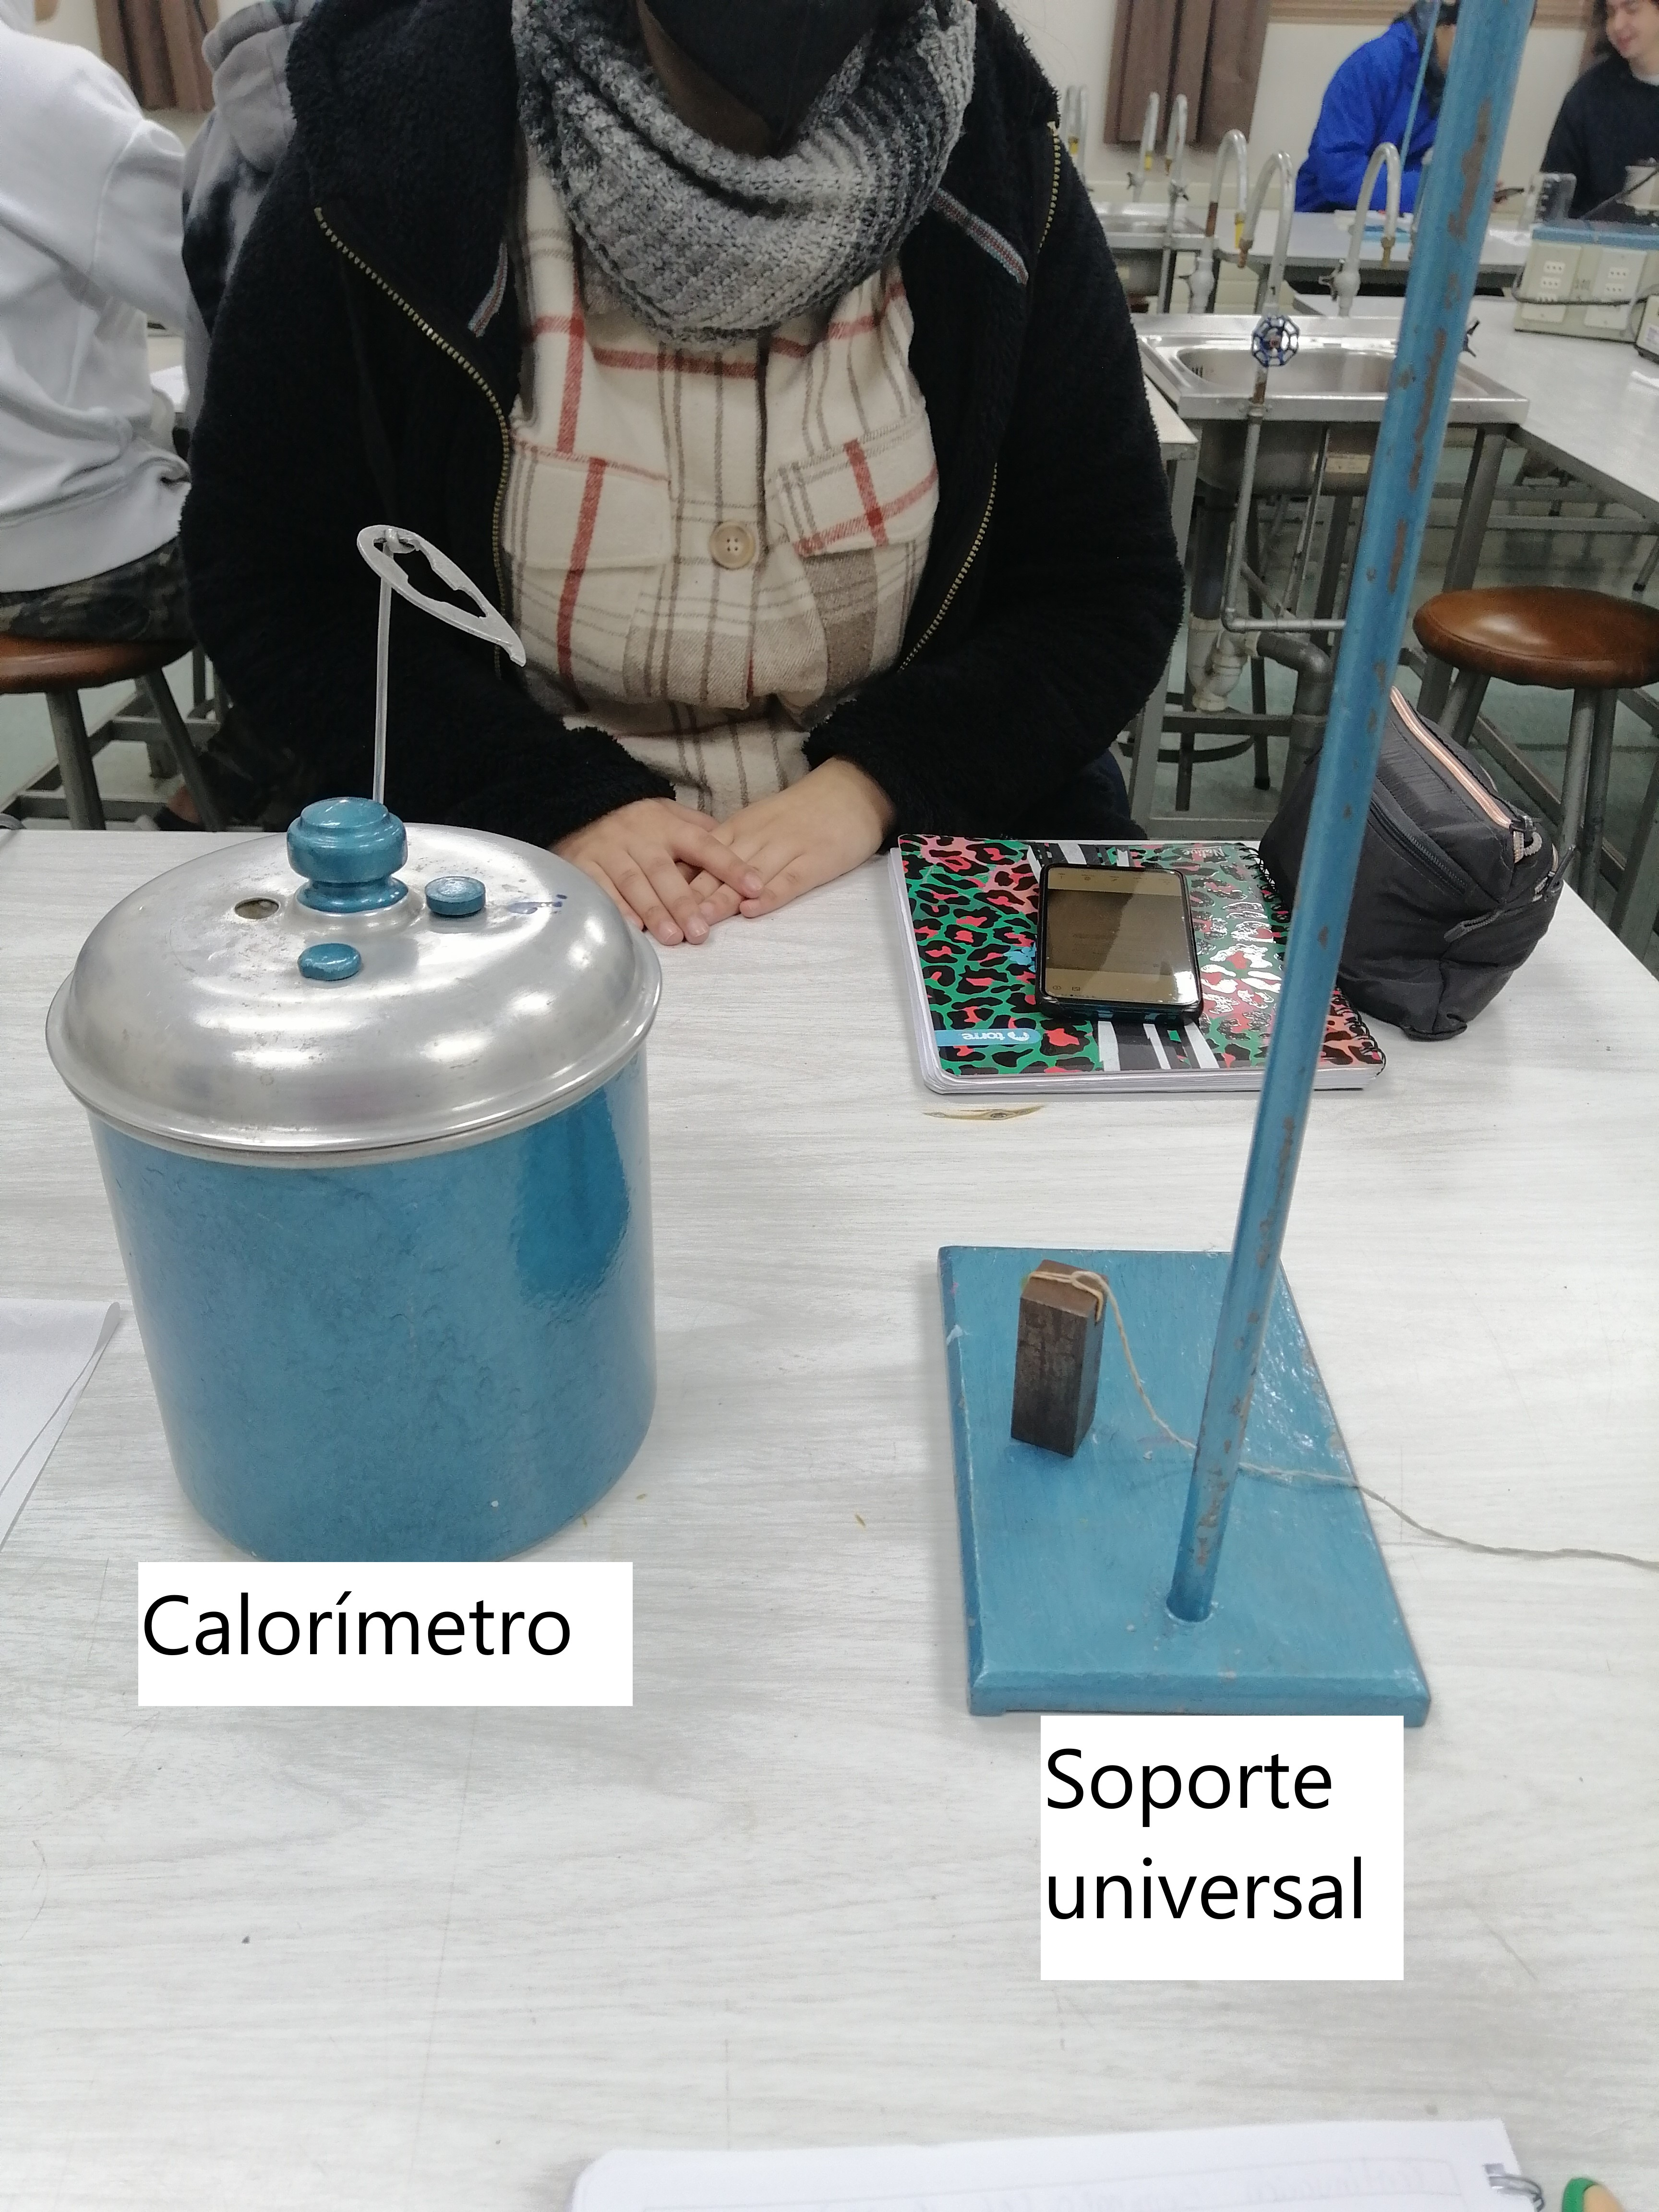
\includegraphics[width=4cm, height=4cm]{img/imag1.jpg}
    \end{subfigure}
    \begin{subfigure}
          \raggedleft
          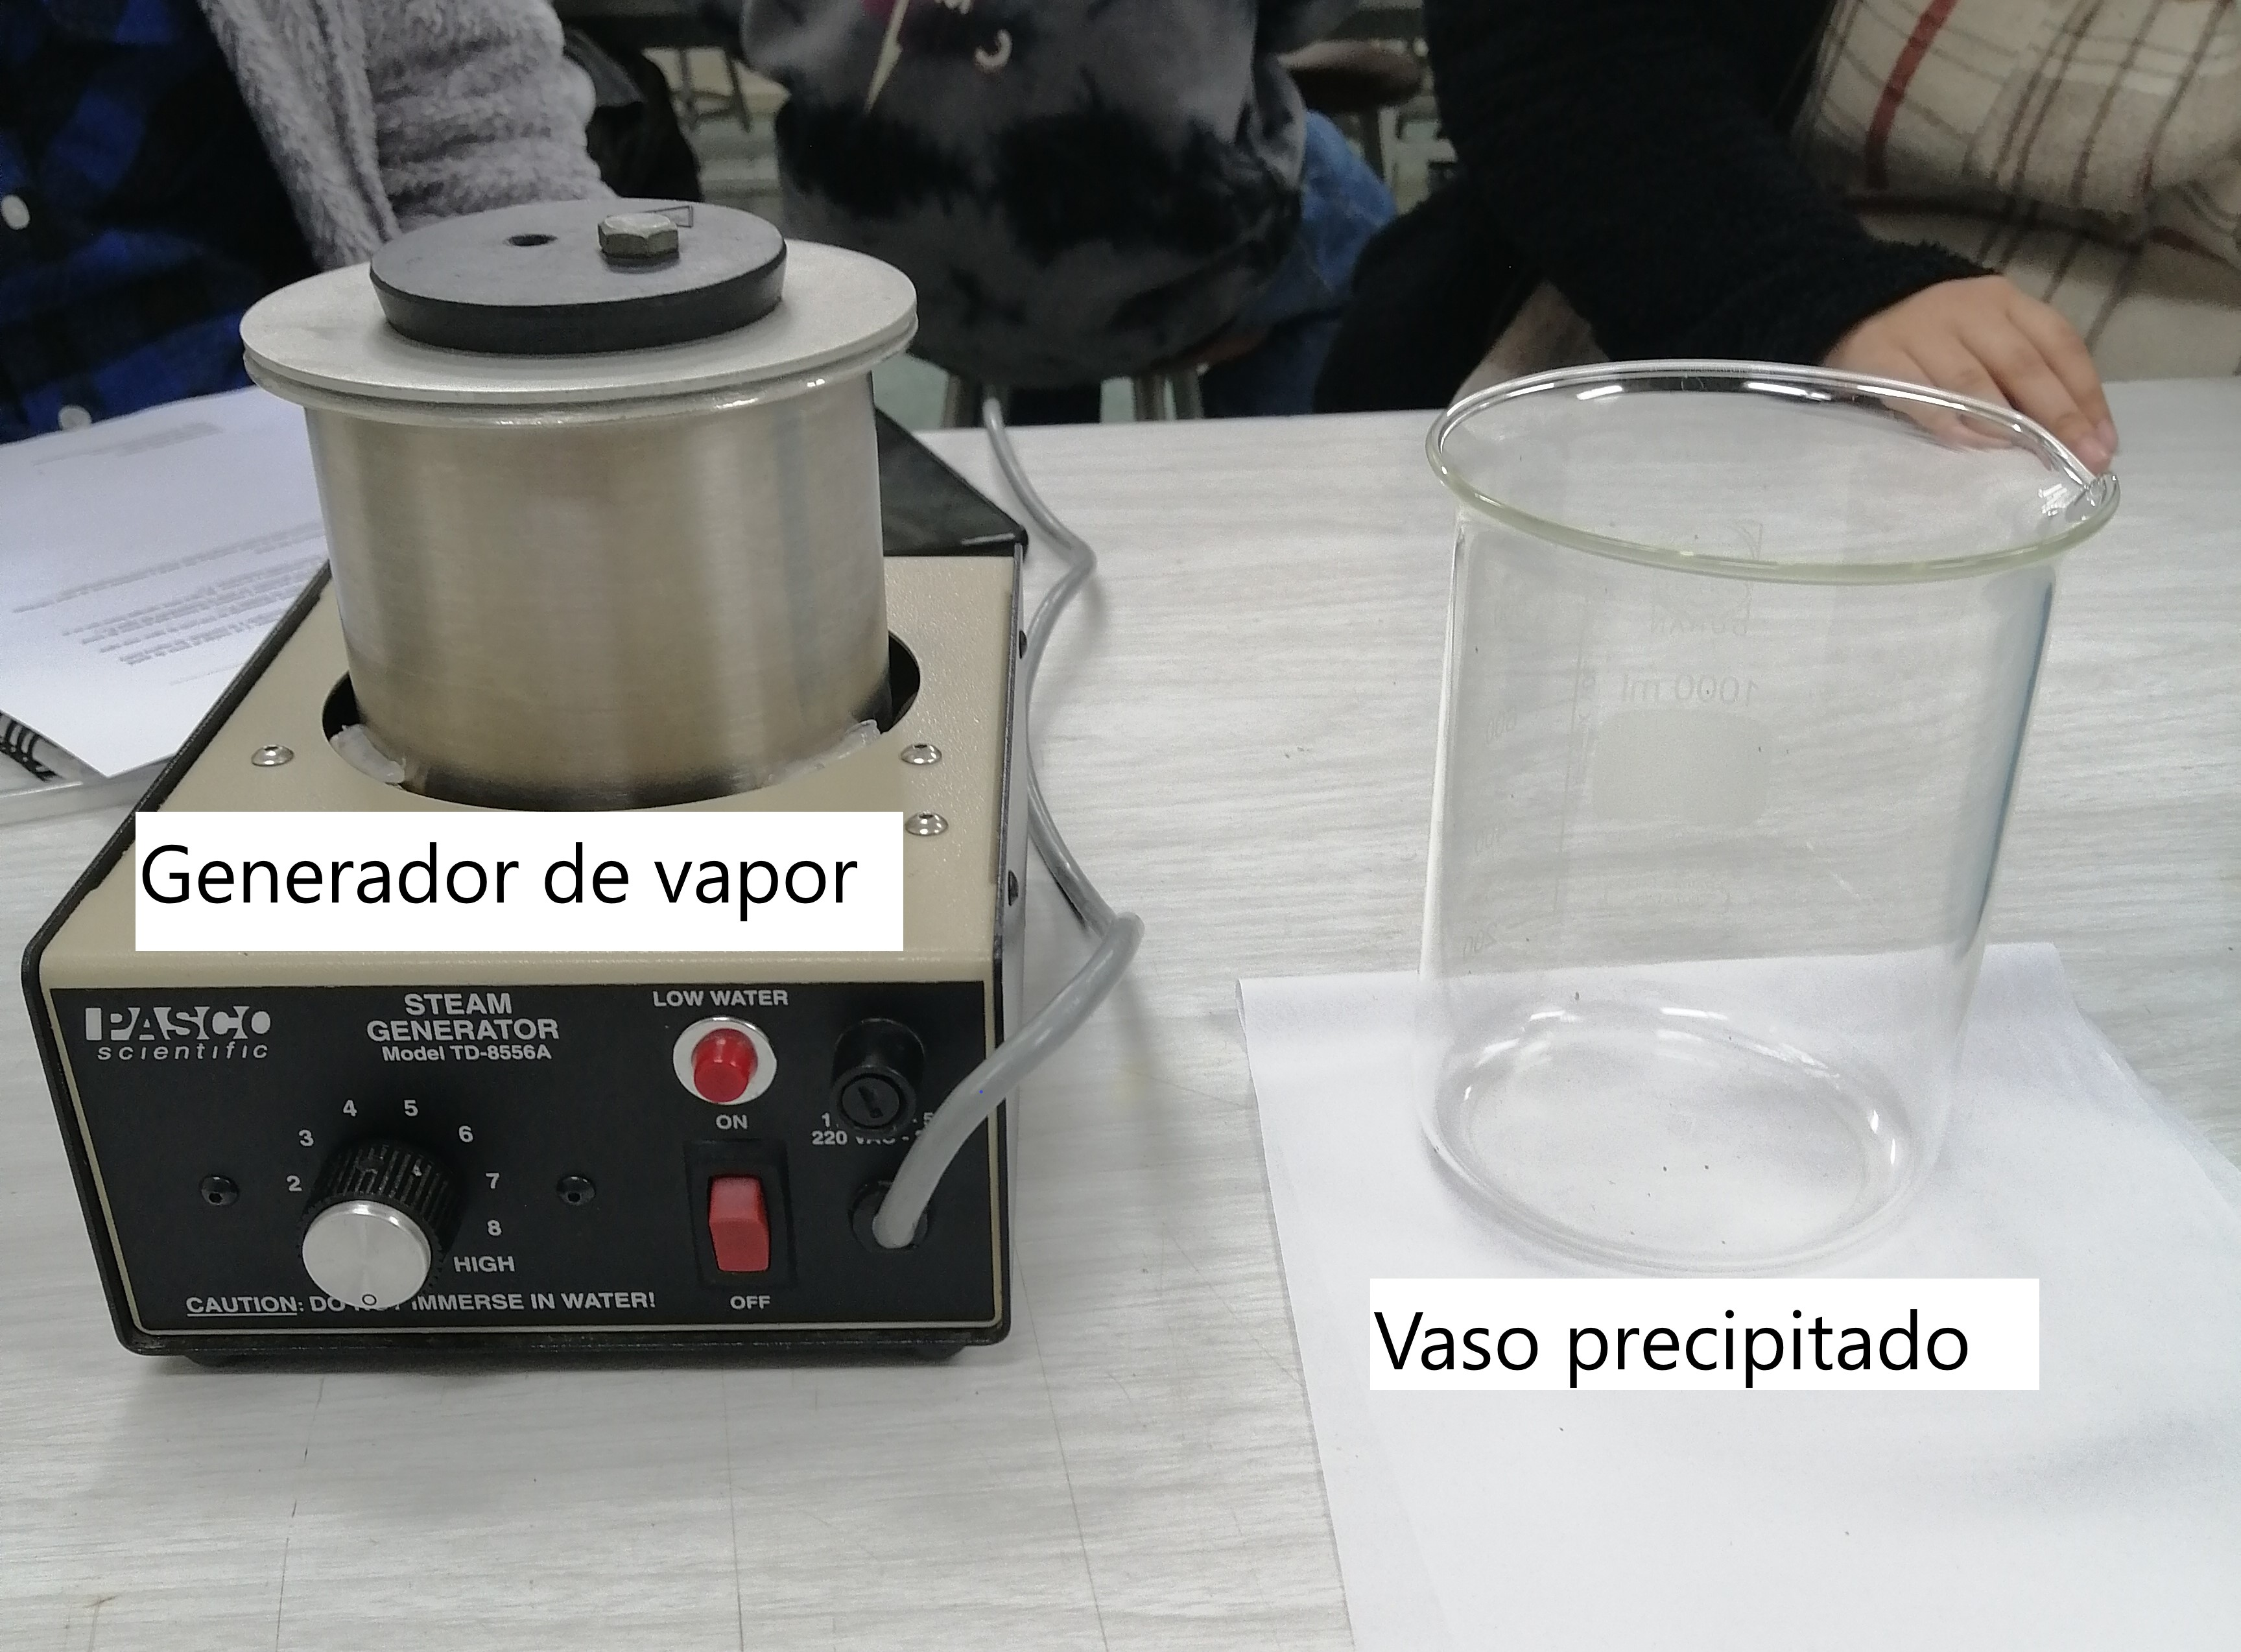
\includegraphics[width=4cm, height=4cm]{img/imag2.jpg}
    \end{subfigure}
    \begin{subfigure}
          \raggedleft
          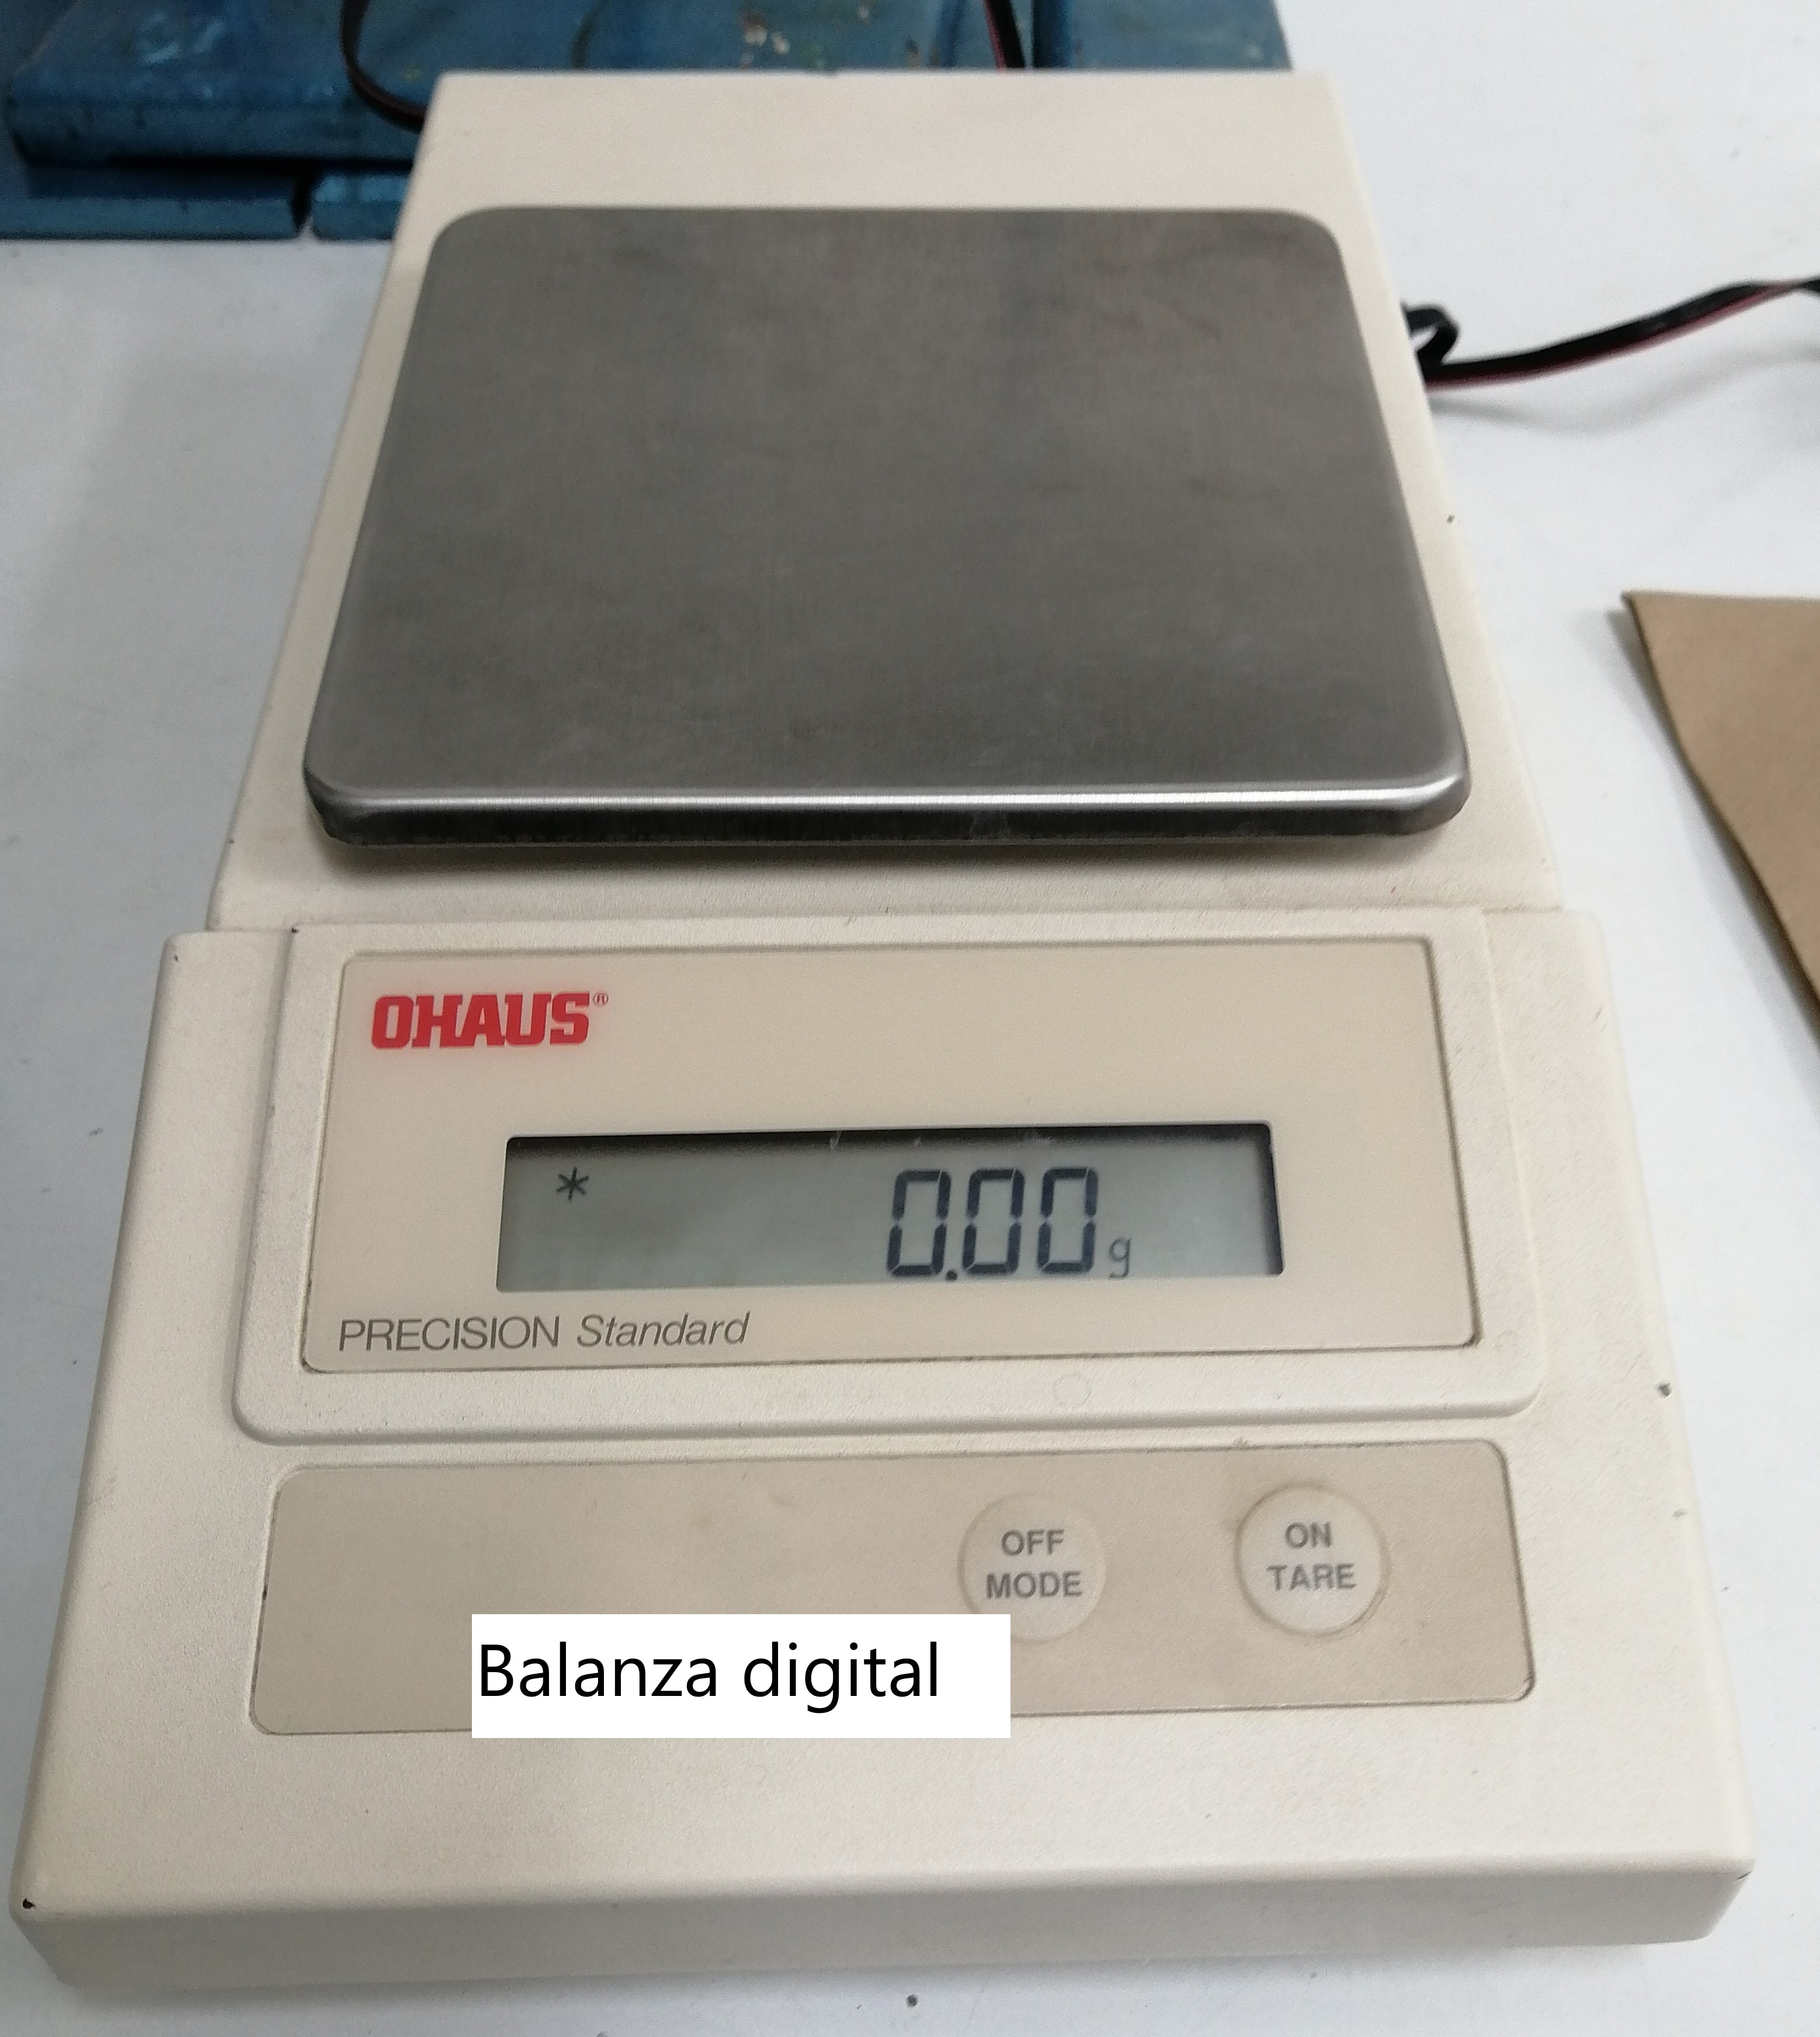
\includegraphics[width=4cm, height=4cm]{img/imag3.jpg}   
    \end{subfigure}   
    \begin{subfigure}
          \raggedleft
          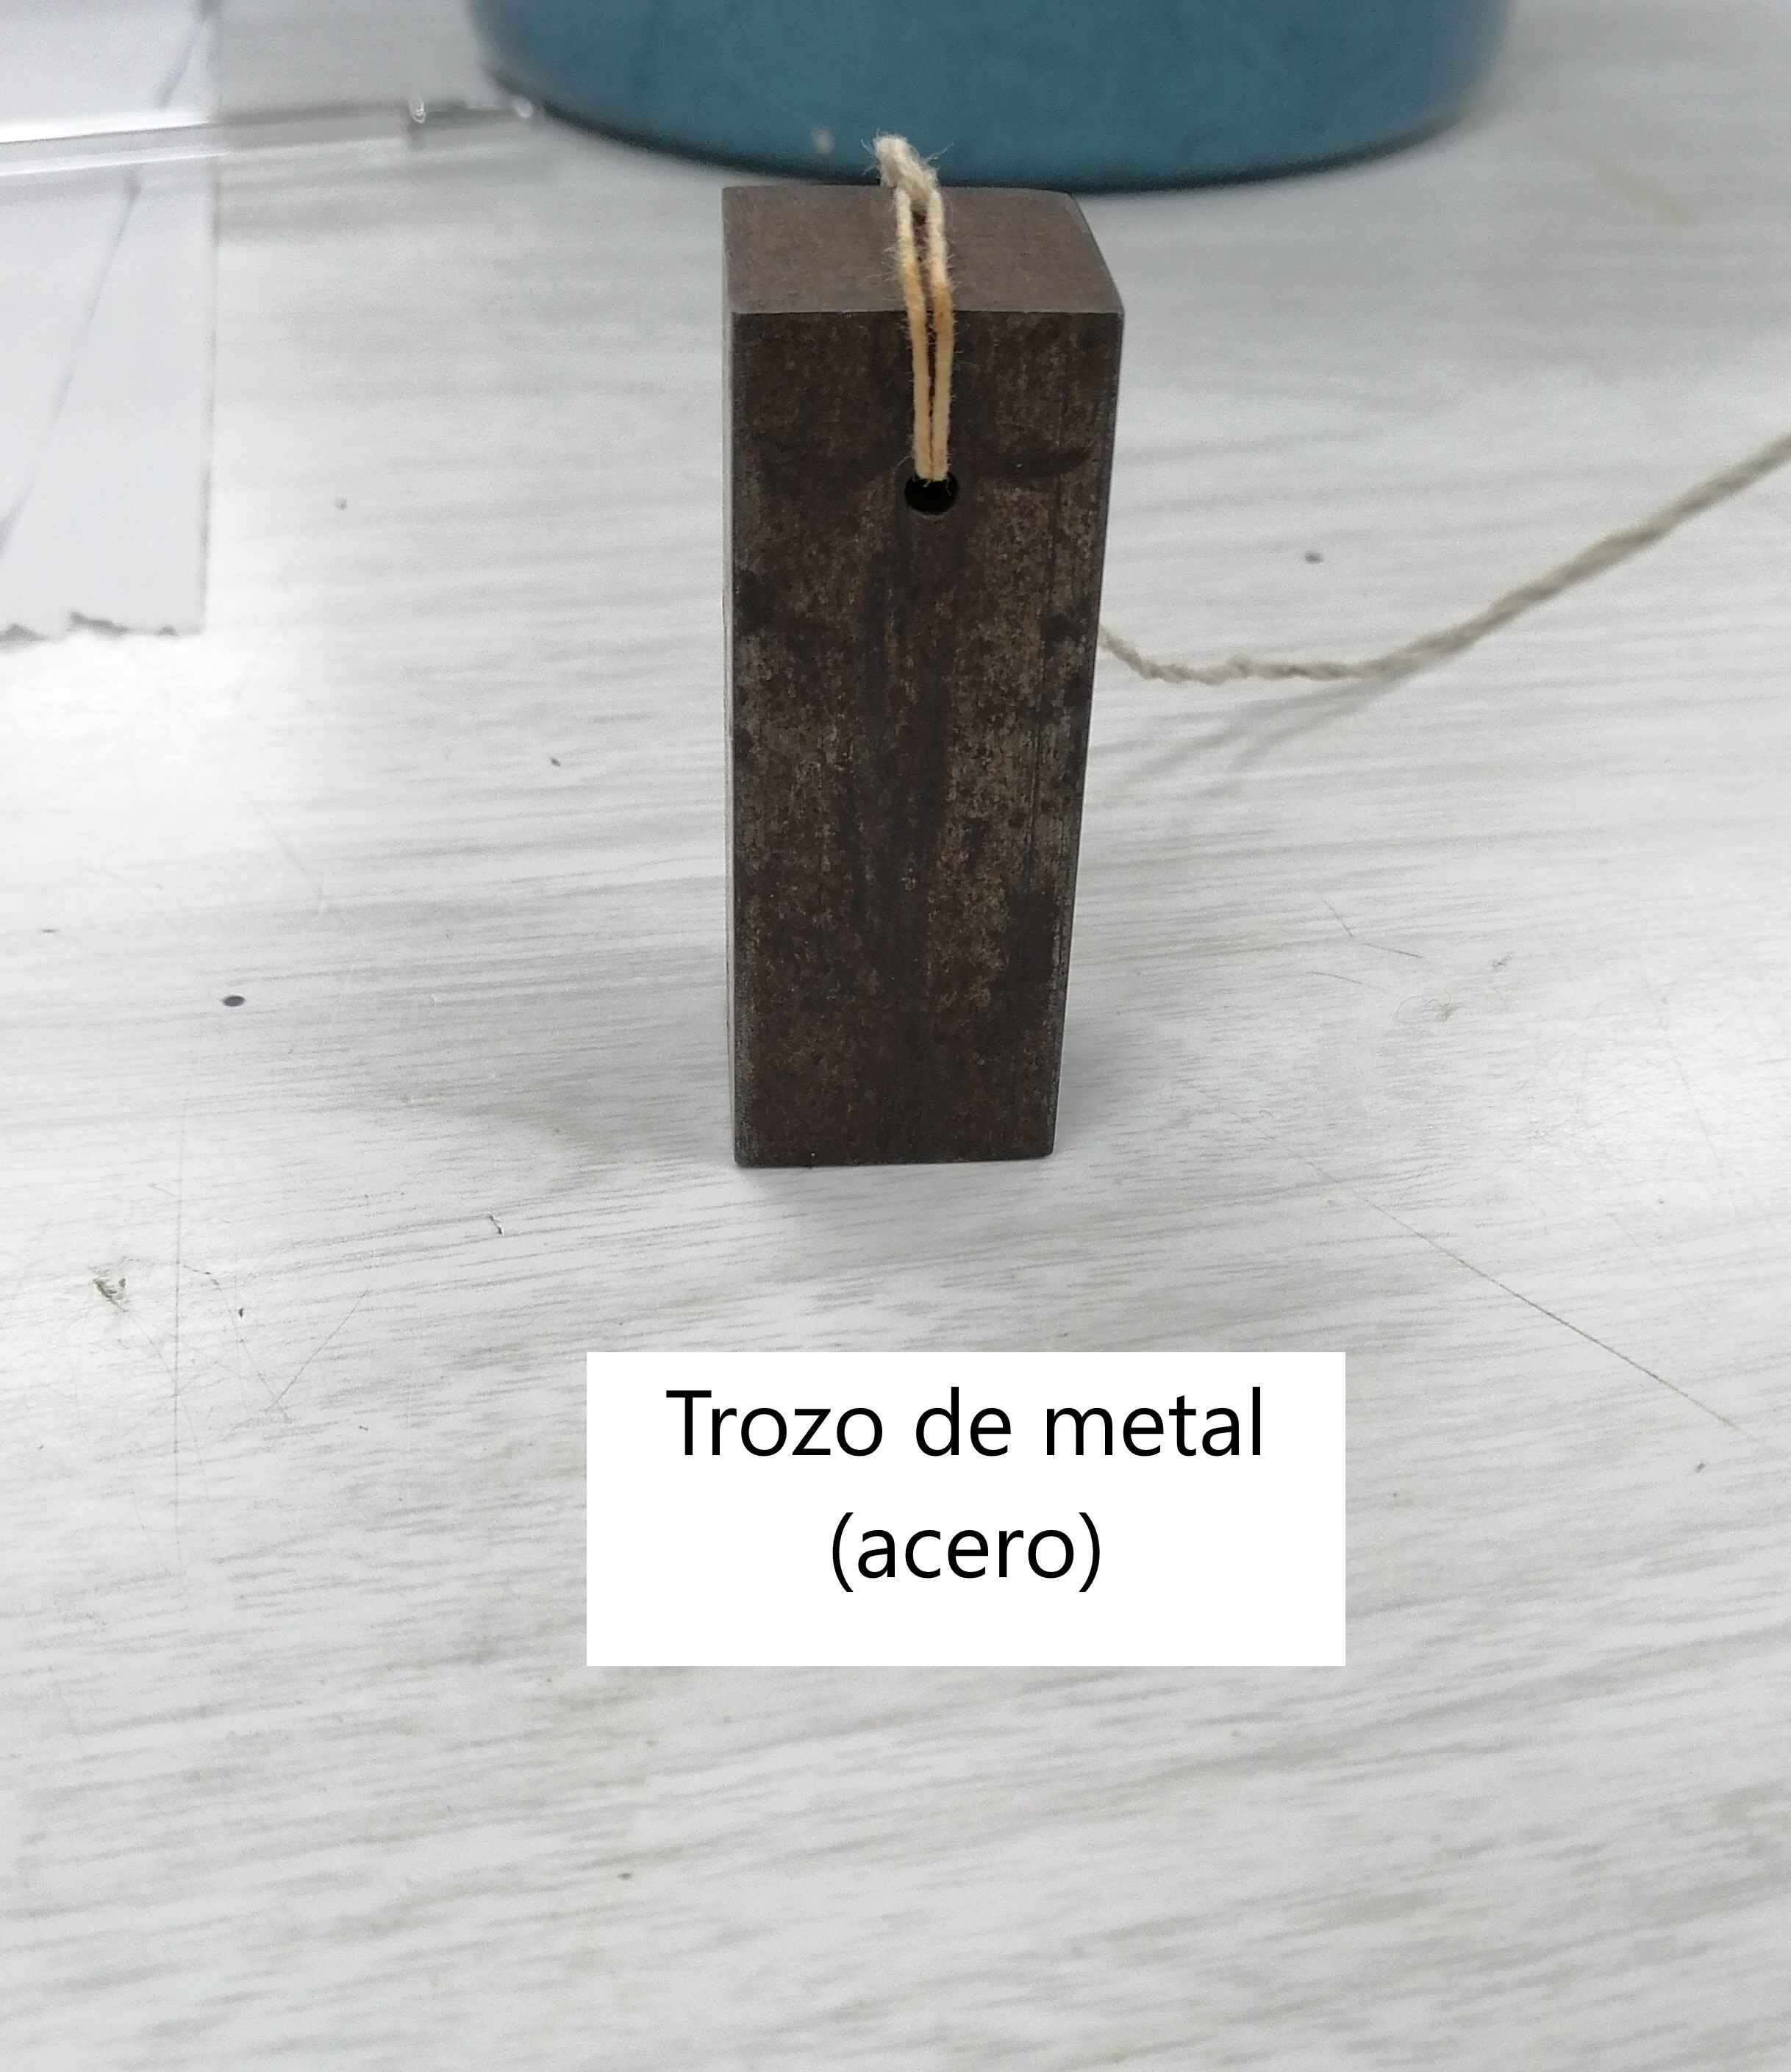
\includegraphics[width=4cm, height=4cm]{img/imag4.jpg} 
    \end{subfigure}
    \begin{subfigure}
          \raggedleft
          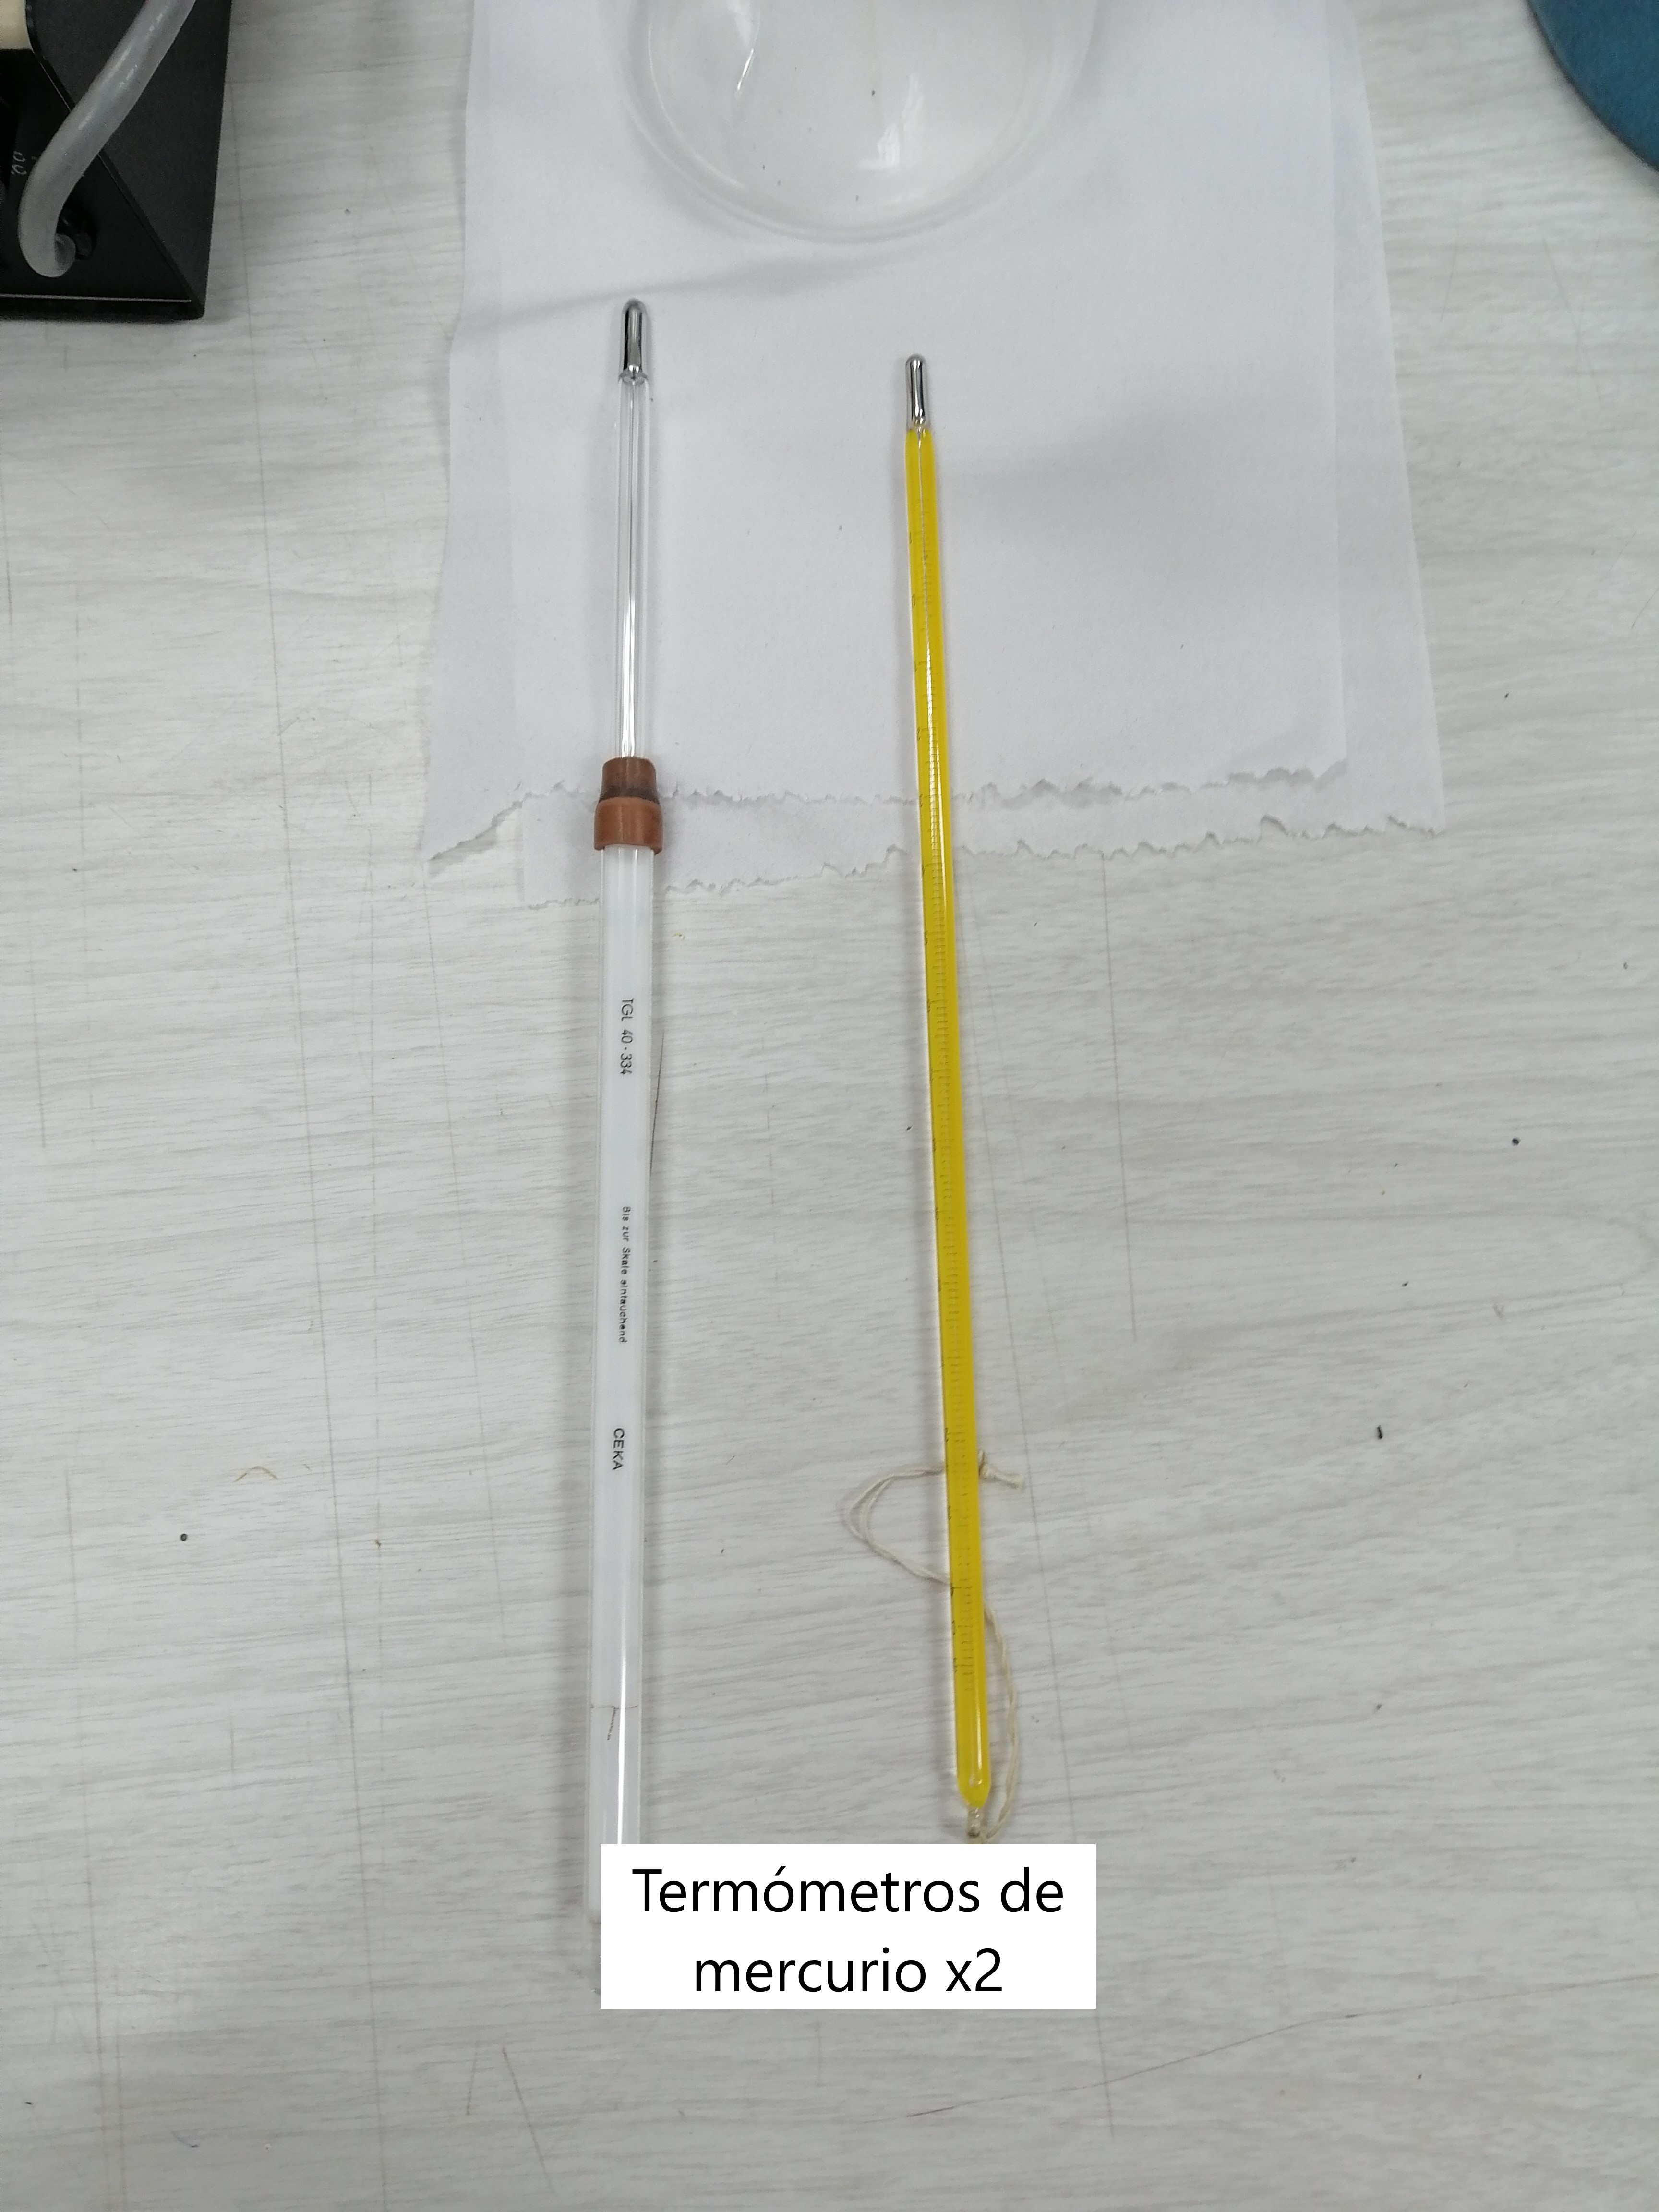
\includegraphics[width=5cm, height=4cm]{img/imag5.jpg} 
    \end{subfigure}
\end{figure}     


\section{Procedimiento}

\begin{itemize}
      \item Se masa el trozo de metal $m_M$.
      \item Se vacían alrededor de $850 [ml]$ de agua en el generador de vapor, y se cuelga el trozo de metal desde el soporte universal,
      de modo que quede totalmente sumergido y se enciende. Esperamos hasta que el agua hierva.
      \item Paralelamente, masamos $350 [ml]$ de agua, $m_a$, luego calculamos su temperatura, $T_{a,i}$ y la vaciamos en el calorímetro. 
      \item Una vez que hierve el agua, se deja encendido hasta por 2 minutos, de forma que el trozo de metal alcance el 
      equilibrio térmico con el agua del generador. Después medimos la temperatura del agua $T_{m,i}$.
      \item Trasladamos el trozo de metal hacía el calorímetro y lo cerramos. Luego, agitamos el agua hasta que al interior se 
      alcance el equilibrio térmico. Por último, medimos la temperatura final, $T_f$.
\end{itemize}

\section{Preguntas}
\begin{enumerate}
    \item Calcular el calor específico $(c)$ del metal.
    \item Colocar el valor de referencia para el calor específico del metal y comparar con el valor calculado (usando error porcentual).
\end{enumerate}


\section{Conclusión}





\begin{thebibliography}{6}
      \bibitem{libro} Sears, F. W., Salinger, G. L. \& Peris, A. J. (2021, 10 enero). Termodinámica, teoría cinética y termodinámica estadística (Spanish Edition) (1.a ed.). Reverte.
      \bibitem{profe} Apuntes del profesor Claudio Faúndez.
\end{thebibliography}













\end{document}
